% siminos/blog/atlas.tex
% $Author$ $Date$

\chapter{Atlas}
\label{chap:atlas}

\begin{description}
\item[2011-11-30 Predrag]
started a new blog, for Predrag's putative letter

\texttt{siminos/atlas/atlas.tex}

\item[2010-07-07 PC]                                    \toCB
A more mathematical thing to fix (not essential if we stick to $\SOn{1}$
case): a clear discussion how the projection of the group tangent version
works for simple Lie groups of dimension higher than $N=1$. It will
involve quadratic Casimir operators, full irreducibility, completeness,
and other such healthy things.

\item[2010-07-12 PC] Now, a more serious thinking,
intellectual
challenge. Rytis and I have started, but not really completed
and written up well a description of how to implement Poincar\'e
section and slice constraints for any continuous Lie symmetry.
Stefan, please study (all references are to the ChaosBook
boyscout version 13.2, Jul 12 2010):
\begin{itemize}
  \item[4.5.1] Stability of Poincar\'e return maps
  \item[5.3] Stability of Poincar\'e map cycles
  \item[13.4] Flows
\end{itemize}
and write your own synthesis of ``Laplace multipliers''
approach to sectioning and slicing a continuous-time
flow with other continuous Lie symmetries. Try first
incorporating $SO(2)$ symmetry as an example, than
a general Lie group $\Group$. Symplectic AKA Hamiltonian
flows are another important class of examples.

\item[2010-07-12 ES]                                \toCB
Stefan I have added data for the $4$ shortest rpo's
in

siminos/CLE/data/CLErpo.dat

It is a plain text file, with tab separated values for the following:

period, angle, initial condition $(x_1,x_2,y_1,y_2,z)$,
Jacobian eigenvalues (5 real numbers)

Let me know if you have trouble importing them and verifying
the period, shift and stability eigenvalues.

Note to self: Tabulate all computed orbits in this human and machine readable format,
rather than Mathematica's own that I use right now.

\item[2011-07-08 Predrag]  Still have to derive the general case: ``
Let $\sliceTan{}$ be a vector normal to the plane of the slice. Then the
dynamics within the slice are given by
\bea
\dot{\gSpace_a}(\sspRed) &=& \frac{\braket{\vel(\sspRed)}{\sliceTan{a}}}
               {\braket{\groupTan(\sspRed)}{\sliceTan{}}}
\continue
\velRed(\sspRed) &=& \vel(\sspRed)
   -\dot{\gSpace}(\sspRed) \cdot \groupTan(\sspRed)
\label{SF:sliceEas1}
\eea
where $\velRed(\sspRed)$ is the velocity in the slice.

  %
We only care about those that are local (and preferably global) {\em
minima}, for which all the eigenvalues of the symmetric matrix
$[N\!\times\!N]$ matrix of second derivatives of distance,
\beq
\frac{\partial^2}
     {\partial \gSpace_a \partial \gSpace_b}
        |\sspRed - \slicep|^2
    =
%  - \braket{\Lg_a e^{\gSpace \cdot \Lg} \ssp}{\sliceTan{b}}=
  - \braket{\groupTan_a(\sspRed)}{\sliceTan{b}}=
  \braket{\sspRed}{\Lg_a \Lg_b\slicep}
\ee{PCinflPoint1}
are positive. In practice we do not need to actually compute this matrix,
we simply pick from among the local minima the infimum of the distance.


 %% ReducTraj*.* - read dasbuch/book/FigSrc/inkscape/00ReadMe.txt
 \begin{figure}
 \begin{center}
  \setlength{\unitlength}{0.40\textwidth}
  %% \unitlength = units used in the Picture Environment
  \begin{picture}(1,0.8361641)%
    \put(0,0){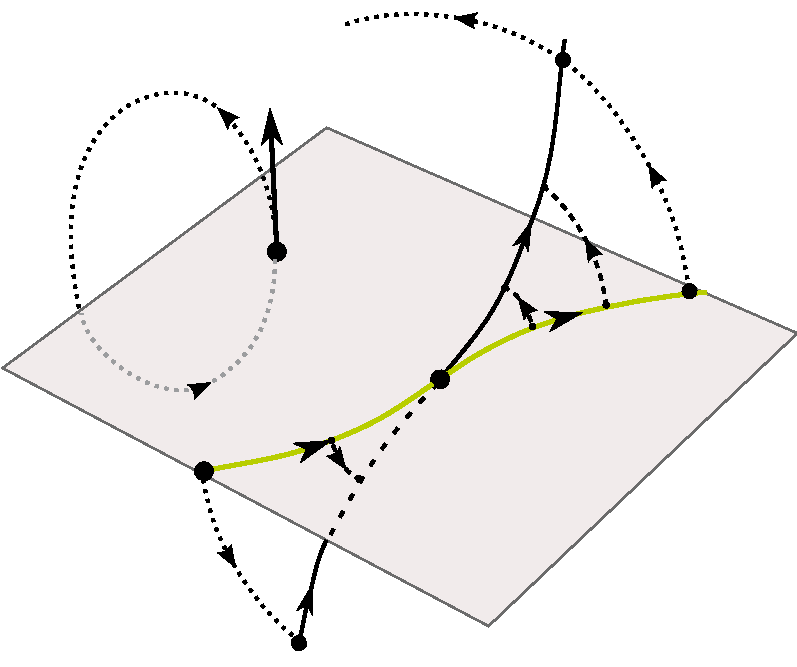
\includegraphics[width=\unitlength]{ReducTraj5.pdf}}%
    \put(0.09054399,0.38282057){\color[rgb]{0,0,0}\rotatebox{-30.34758661}{\makebox(0,0)[lb]{\smash{$\pSRed$}}}}%
    \put(0.57768586,0.29773425){\color[rgb]{0,0,0}\rotatebox{0.0313674}{\makebox(0,0)[lb]{\smash{$\sspRed(0)$}}}}%
    \put(0.59310014,0.69932675){\color[rgb]{0,0,0}\rotatebox{0.03136739}{\makebox(0,0)[lb]{\smash{$\ssp(\tau)$}}}}%
    \put(0.8268425,0.39772328){\color[rgb]{0,0,0}\rotatebox{0.03136739}{\makebox(0,0)[lb]{\smash{$\sspRed(\tau)$}}}}%
    \put(0.81220962,0.66529577){\color[rgb]{0,0,0}\rotatebox{0.03136739}{\makebox(0,0)[lb]{\smash{$\LieEl(\tau)$}}}}%
    \put(0.23150193,0.63610779){\color[rgb]{0,0,0}\rotatebox{0.0313674}{\makebox(0,0)[lb]{\smash{$\LieEl\,\slicep$}}}}%
    \put(0.37740434,0.49597258){\color[rgb]{0,0,0}\rotatebox{0.0313674}{\makebox(0,0)[lb]{\smash{$\slicep$}}}}%
    \put(0.3627714,0.69665188){\color[rgb]{0,0,0}\rotatebox{0.0313674}{\makebox(0,0)[lb]{\smash{$\sliceTan{}$}}}}%
  \end{picture}%
 \end{center}
 \caption{\label{fig:ReducTraj}
 % (b)
\Slice\ \pSRed\ is a hyperplane \refeq{PCsectQ}
passing through the {\template} point $\slicep$,
and normal to the group tangent $\sliceTan{}$ at $\slicep$.
It intersects all
group orbits (indicated by dotted lines here) in an open
neighborhood of $\slicep$.  The full
\statesp\ trajectory $\ssp(\tau)$ and the \reducedsp\
trajectory $\sspRed(\tau)$ belong to the same group orbit
$\pS_{\ssp(\tau)}$ and are equivalent up to a group rotation
$\LieEl(\gSpace)$, defined in  \refeq{sspOrbit}
(from \wwwcb{}).
 }%
 \end{figure}
													\toCB
Ponder whether to use \reffig{fig:ReducTraj} (current, but not updated
yet), or Fig~{fig:slice} in ChaosBook.org
How it was drawn is described in
\\
dasbuch/book/FigSrc/inkscape/00ReadMe.txt

\item[2011-07-08 Predrag]
The $L^2$ norm of $\groupTan(u)$ is weighted by
the quadratic Casimir \refeq{QuadCasimir}. For \SOn{2} this is
$C_2^{(m)} = m^2$,
\beq
\oint \frac{d\gSpace}{2\pi}
     \, (\Lg u(\gSpace))^T \Lg u(2\pi-\gSpace)
= \sum_{m=1}^\infty m^2 \left(a_m^2 + b_m^2\right)
\,.
\ee{tangL2norm1}


\item[2011-07-08 Predrag]
Ridges are of Lebesgue measure zero, no way you would hit them.

We do not need to be very precise about the instant
where we switch, as long as we are away from either slice's singularity
subspace.


\item[2011-07-08 Predrag, from \refref{FrCv11}]                     \toCB
At this point it is worth noting that imposing the global and fixed slice
%\refeq{PCsectQ}
is not the only way to separate equivariant dynamics into `group
dynamics' and `shape' dynamics\rf{BeTh04}. In modern mechanics and even
field theory (where elimination of group-directions is called
`gauge-fixing') it is natural to separate the flow {\em locally} into
group dynamics and a transverse, `horizontal'
flow\rf{Smale70I,AbrMars78}, by the `method of
connections'\rf{rowley_reduction_2003}. From our point of view, such
approaches are not useful, as they do not reduce the dynamics to a
lower-dimensional \reducedsp\ $\pS/\Group$.

\item[2010-09-28 ES: Faddeev-Popov ghosts]                    \toCB
(moved to here from froehlich/blog)
\\
From my random readings, supposedly making up for my inability to attend
colloquia in French: Faddeev in a
\HREF{http://www.scholarpedia.org/article/Faddeev-Popov_ghosts}{scholarpedia
article} discusses the difficulties in Yang-Mills quantization that led
him and Popov to introduce fictitious fields, now known as
\emph{Faddeev-Popov ghosts}. The problem was that of gauge fixing,
essentially of working on a slice. Faddeev says:

\begin{ttfamily}
It was clear that the equivalence principle had to be taken into account.
In the functional integral framework, the equivalence principle implies
that one has to integrate over classes of gauge equivalent fields instead
of integrating over all fields $A_\mu^a$.

The choice of the representatives in the classes of equivalent fields is
realized by means of a gauge condition (gauge fixing), for instance,
\[
    \partial_{\mu} A_{\mu}^{a} = 0 .
\]
This condition defines a plane in the set of all fields, which is
intersected by the gauge orbits defined by
\[
    A_{\mu} = A_{\mu}^{a}t_{a} \to A_{\mu}^{\Omega}
            = \Omega A_{\mu} \Omega^{-1} + \partial_{\mu} \Omega \Omega^{-1} .
\]
In this context, the difference among abelian and non-abelian cases
becomes clear. In the abelian case, we take $\Omega(x) =
\exp{i\Lambda(x)}$ and a gauge orbit is defined by
\[
    A_{\mu} \to A_{\mu} + \partial_{\mu} \Lambda ,
\]
which is just a linear shift. Thus all the abelian orbits intersect the
gauge surface at the same angle.

In the non-abelian case, the gauge orbit equations are non-linear and the
intersection angle depends on the field parameterizing the orbit. It is
clear that this must be taken into account in the functional integral.
\end{ttfamily}

See the wikipedia link to put this in the proper context. As an abelian
case Faddeev lists quantum electrodynamics where the group is $U(1)$ (the
same as in \cLe\ if we think in terms of complex variables). As a
non-abelian example he lists the Standard Model: $U(1)\times SU(2) \times
SU(3)$.

Faddeev relies on the group being connected to write group action in
exponential form, as Stefan does. $\On{2}$ in Kuramoto-Sivashinsky is
non-abelian so I am worried that there might be more work required. Are
all non-connected compact Lie groups non-abelian and vice versa?

The weight factor Faddeev and Popov introduced might be helpful in
trace-formulas for non-abelian groups.

\item[2011-12-06 Roman] However,  ECS can be used to project
trajectories onto a low-dimensional visualization where coordinates $a^k_{i}(t)$
are defined by the inner product
\beq
\label{coordinatesRG}
a^k_{i}(t)= \frac{1}{V} \int_V {\bf e}^k_i(t)^\dagger\cdot({\bf u}(t)-{\bf u}^k(t)) dV,
\eeq
%\pagebreak
where $V$ is the flow domain volume, ${\bf u}^k(t)$ is the ECS closest to
the system state at time $t$, and ${\bf e}^k_i(t)$ are basis functions
representing a set of unstable and weakly stable modes characterizing the
particular ECS.

\item[2011-12-06 Predrag]
Mhm - why are we introducing new notation for \statesp\
coordinates in \refeq{coordinatesRG}? I cannot imagine a situation in which one
would like to make the bases  ${\bf e}^k_i$ time dependent, ${\bf e}^k_i(t)$,
and we mostly use ECS themselves to construct projections, as in
\reffig{f:ssptransient}, not their stability eigenvectors. If you are really
thinking of using ECS's ${\bf u}^k(t)$ as templates whose linearized local
charts compose a global atlas for the flow, they would not be time dependent,
but fixed by a set of Poincar\'e sections to \statesp\ points ${\bf u}^k$, and
the associated set of unstable and weakly stable eigenvectors (what are
"modes"?) ${\bf e}_i^k$ would also be confined to the Poincar\'e section, and
not time dependent. But I think this is way too sophisticated for referees to
wrap their heads around....

I propose you drop time dependence from ${\bf e}^k_i(t)$ and ${\bf
u}^k(t)$ and pass over all that in silence for now. Or perhaps keep the
formula as is, as neither the authors themselves have never sorted out
how the \po\ eigenvectors are to be used in practice.

\begin{figure}
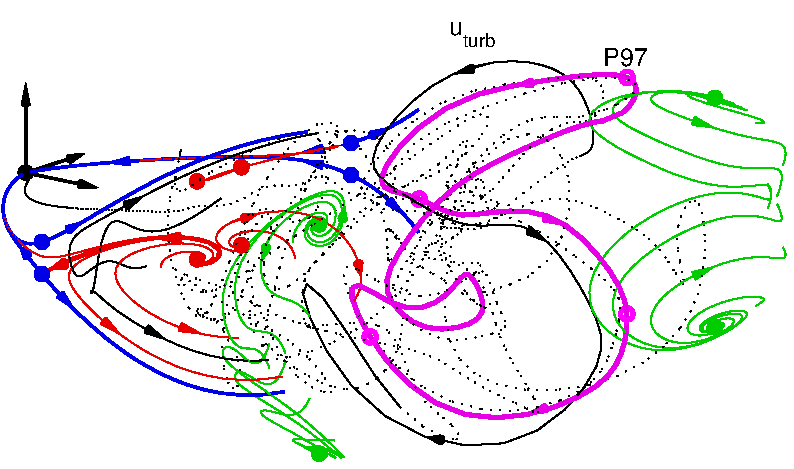
\includegraphics[width=\textwidth]{P97portrait5}
\caption{
{\bf A state-space portrait of turbulent plane Couette flow.}
A turbulent trajectory ${\bf u}_{\text{turb}}$ (solid and dotted black
lines) shadowing the P97 periodic orbit (bold magenta line) and the
unstable manifolds (blue, red, and green lines) of symmetry-related
equilibria (solid blue, red, and green dots; the black dot at the origin
is the laminar flow state). Velocity fields corresponding to the open
magenta dots on P97 are shown in  reffig~{f:ssptransient2}. Dynamic
connections are shown as bold red and blue lines connecting different
equilibria (filled dots).
}
\label{f:ssptransient}
\end{figure}

\item[2011-12-06 John] Predrag's comment on \refeq{coordinatesRG} is on
target: it makes sense with the verbal description attached to it, but
the time-dependence of the basis set $e_i^k(t)$ and the nearest ECS
$u^k(t)$ is pretty confusing. The bigger problem is that the equation as
is reflects what we want to do, but doesn't the projection in
\reffig{f:ssptransient}, which uses a fixed basis based on four
symmetry-related ECS to produce a global portrait.

\item[2012-02-21 PC]  I like the way this chaos class is working, and I
think we can put together some of the best class contributions into a
pedagogical article about sections and slices. And we have a chance to
publish this in a high quality issue of one of the better journals in the
field, Chaos:

\item[2012-02-21 Phil Holmes to PC]
We write in connection with the recent IUTAM Symposium on 50 Years of
Chaos: Applied and Theoretical, held in Kyoto, which you attended. In
addition to the Conference Proceedings to be published by Elsevier as
part of their regular IUTAM series, the American Institute of Physics
(AIP) has agreed to devote a special issue of the AIP Journal
\emph{Chaos} to papers representing a selection of the topics presented.
This is planned to appear as \emph{Vol 22 (4), December 2012}. So far 11
invitees have agreed to contribute papers; only one (David Ruelle) has
declined.


Based on your interesting presentation in Kyoto, we would like to invite
you to submit a paper for consideration for this special issue of Chaos.
Please let us know as soon as possible if you would like to do so, at the
latest, before Monday Jan 16th, 2012. Papers may either review a topic,
preferably including new results, or present entirely new, unpublished
results; papers should also reflect the topics and themes presented at
the symposium. All contributions will be refereed in the usual manner, as
for unsolicited submissions to AIP journals. At present we expect this to
require submission of the paper by \textbf{March 30th, 2012}, with
resubmission of revised papers during June 2012.


\textbf{[NOTE from Phil Holmes]}
Since some of the work you described has appeared in previous papers, in
particular that on channel flows with John Gibson, I would be especially
interested in the new results on symmetry groups hinted at in your
presentation.


\item[2012-02-21 PC to Phil Holmes]
Thank you for your kind invitation to contribute to the special issue of
the AIP Journal Chaos in connection with our "50 Years of Chaos". I am
sorry I am responding past your deadline, but I was not sure we would
have results interesting enough to report in this issue, results that
have not been written up for other publications. Now I am feeling more
confident that we can offer a novel pedagogical review of the symmetry
reduction by the method of slices (that I had described by its
application to one example, the pipe flows, in Kyoto), so I would like to
join this very fine group of contributors to the planned December 2012
Chaos.

\item[2012-02-23 PC] For instructions read
\texttt{siminos/atlas/Chaos-v1/00ReadMe.txt}. The deadline is

\textbf{April 16, 2012}

\item[2012-02-18 Predrag] clippings

This procedure has been devised by Poincar\'e in the context of celestial
mechanics, in the aim of reducing the analysis of long-term planetary
motion and its dynamic stability [Poincar\'e, Les m\'ethodes nouvelles de
la m\'ecanique c\'eleste 1892].

\begin{figure}
  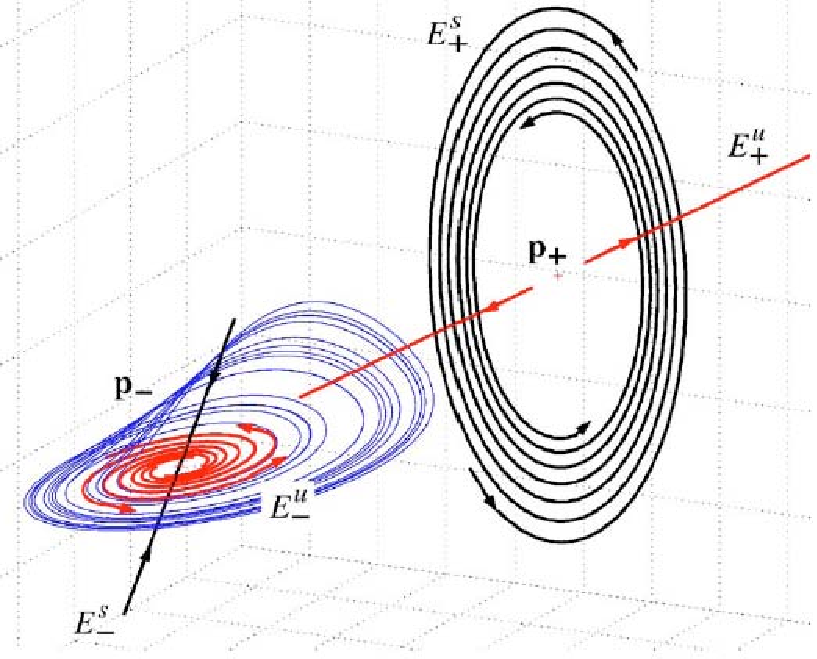
\includegraphics[width=0.6\textwidth]{AmLeAg06Im1}\\
  \caption{From \refref{AmLeAg06}:
R\"ossler attractor with fixed points and their manifolds. The linear
stable manifold at the lower fixed point is 1-dimensional and the
unstable one is associated with an unstable focus. The stable manifold at
upper fixed point is a stable focus and the unstable manifold is
1-dimensional}
\label{fig:AmLeAg06Im1}
\end{figure}

From \refref{AmLeAg06}:
``A linear system is $\dot{x} =Ax$ and an affine system is $\dot{x}
=Ax+b$, where $A$ is a constant matrix and $b$ is a constant vector.''

                                            \toCB
Draw (un)stable eigenvectors as in \reffig{fig:AmLeAg06Im1}.
``
In the R\"ossler system, the switching is induced by the
nonlinearity which acts when the trajectory is sufficiently far
from lower fixed point, that is, beyond the threshold $x-c$ in
the third equation. The nonlinearity
acts when the trajectory is sufficiently close to upper fixed
points where its converging spiral induces the folding by
sending the trajectory back to the neighborhood of lower fixed
point along its unstable manifold. Thus, the lower fixed point
is mainly responsible for the stretching and upper fixed point for
the folding.
''

\end{description}
